\titlespacing*{\subsection}{0pt}{1.0em}{0.3em}
\titlespacing*{\paragraph}{0pt}{1.0em}{0.3em}

\subsection{문제 정의 및 개요}
본 연구는 여러 환율 및 거시경제 시계열이 상호 의존적인 구조를 가진다는 점에 주목하여, 변수 간 상호의존성과 시간적 의존성을 동시에 학습하는 그래프 기반 시계열 예측 문제를 다룬다. 이러한 문제를 해결하기 위해 다변량 시계열 간 잠재적 상호의존을 학습하기 위해 B-MTGNN 기반 모델을 적용한다~\cite{Wu2020MTGNN}.
각 국가의 통화 집합을 $C=\{c_1,c_2,\dots,c_N\}$라 하면, 각 변수는 그래프의 노드로 표현된다. 관측 시점 $t=1,\dots,T$ 동안 시계열 데이터 주어졌을 때, 목표는 다음의 조건부 예측분포를 추정하는 것이다.
\begin{equation}
p\!\left(\mathbf{Y}_{T+1:T+H}\mid \mathbf{X}_{1:T},G\right)
\tag{1}
\end{equation}
여기서 $H$는 예측 구간이며, $\mathbf{Y}_{T+1:T+H}$는 미래 $H$스텝의 예측 대상 시계열 백터이다. 이 정의는 단일 시점의 점 예측이 아니라, 미래 경로 전체에 대한 확률적 예측을 의미한다. 즉, 모델은 과거 시계열 입력 $\mathbf{X}_{1:T}$와 변수 간 상호의존 그래프 $G$를 조건으로 하여 미래 시계열 $\mathbf{Y}_{T+1:T+H}$의 조건부 확률분포 $p(\mathbf{Y}_{T+1:T+H}\mid \mathbf{X}_{1:T},G)$를 추정한다. 구체적인 학습 및 예측 구간의 설정은 4장의 실험 환경에서 서술한다.

\begin{figure*}[!ht]
\centering
\scalebox{1}[1.2]{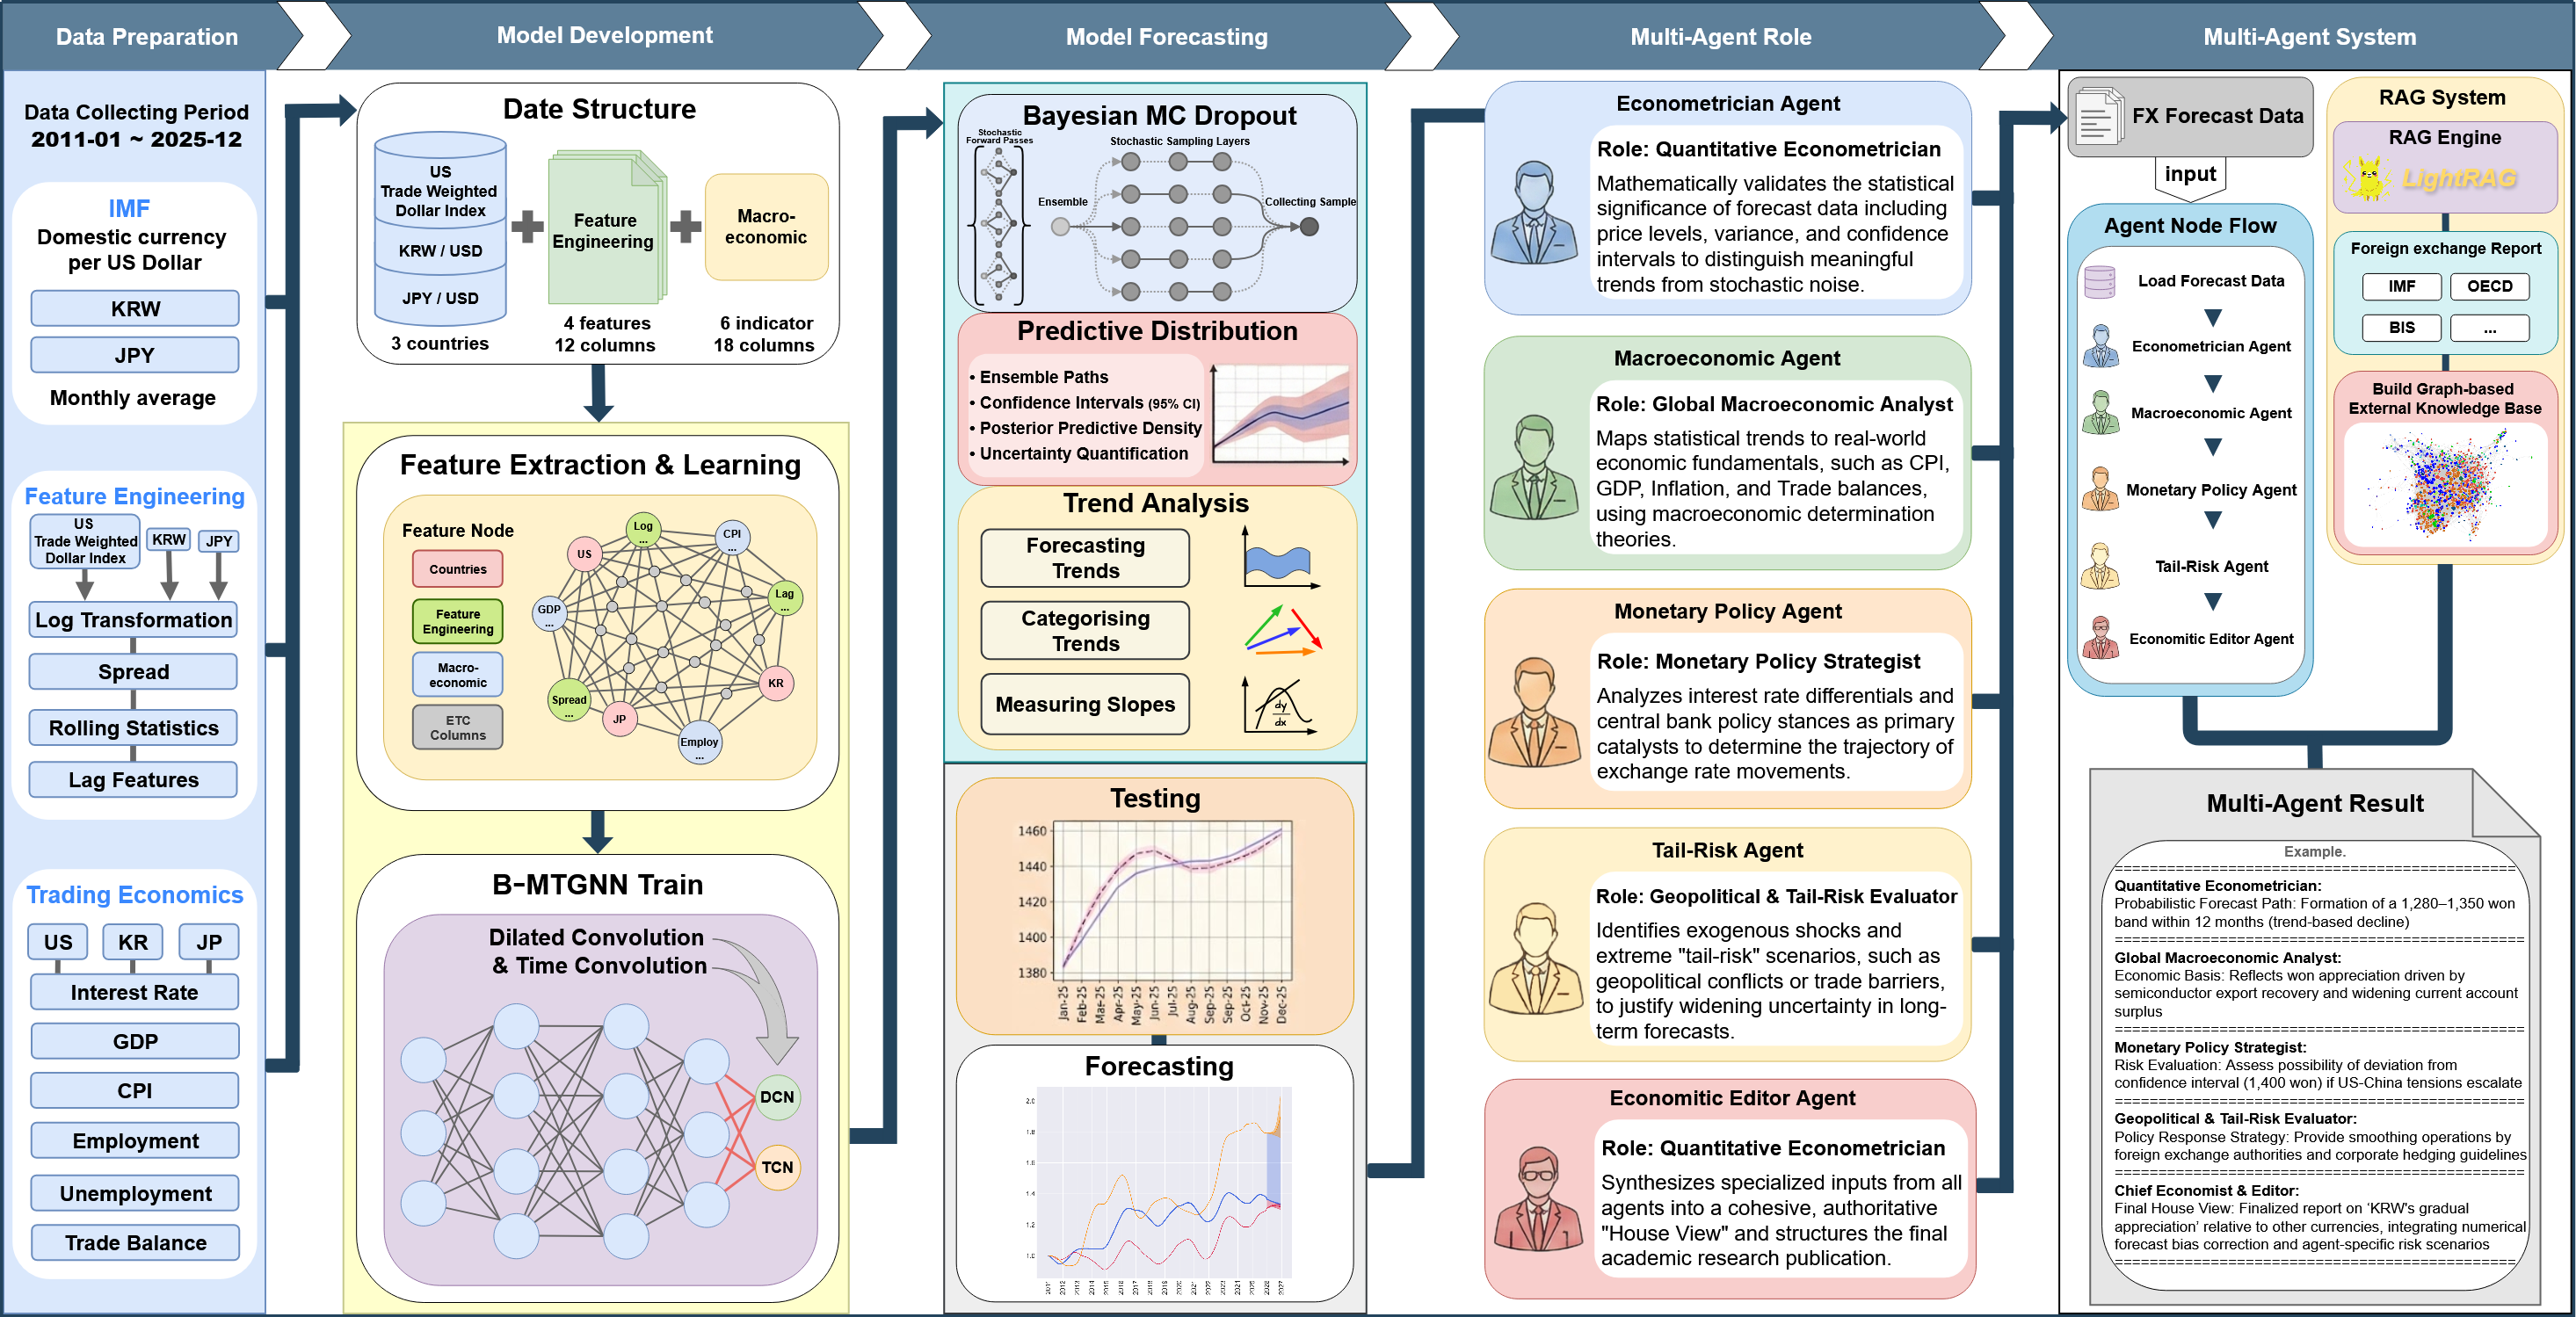
\includegraphics[width=\textwidth]{figure/fx_framework.drawio.png}}
\caption{국가 간 환율 변동 구조 예측을 위한 AI 프레임워크: 다변량 시계열 데이터, B-MTGNN 기반 예측, 추세–격차 분석, 멀티 에이전트 검증을 통합하여 전략적 외환 분석 결과 해석}
\label{fig:framework}
\end{figure*}

\subsection{입력 변수 및 정보 구성}
환율은 단일 요인으로 움직이지 않으며, 환율 자체의 변동 구조와 국가 간의 상호작용에 따라 서로 영향을 주며 함께 변한다. 이에 따라 본 연구는 각 국가 $i$에 대해 다음의 구성요소를 결합한다. 국가 $i$의 환율 관측을 $E_i(t)$라 할 때, 모델의 기초 입력이 되는 로그 수익률을 $Y_i(t)$로 정의한다.
% 기초입력이 로그 수익률?
\begin{equation}
Y_i(t)=\log E_i(t)-\log E_i(t-1)
\tag{2}
\end{equation}
본 연구에서는 딥러닝 모델의 학습 안정성을 위해 $Y_i(t)$를 환율 상태로 정의한다. 모델이 국가 간 단기 흐름과 함께 움직이는 패턴을 명시적으로 포착할 수 있도록, 특성 공학을 통한 입력 변수 가공으로 과거 수익률 값, 국가 간 수익률 격차, 그리고 롤링 상관계수를 파생 지표 $F_i(t)$ 집합으로 포함하였다. 이와 함께 국가 경제에 구조적 영향을 미치는 정책 금리, GDP, 소비자물가지수, 고용 지표, 실업률, 무역 수지 등의 주요 거시·금융 지표를 $M_i(t)$로 둔다. 최종적으로 국가 $i$의 시점 $t$ 입력 다변량 특징 벡터는 다음과 같이 수식화된다.
% Feature engineering 직접 언급
\begin{equation}
\mathbf{x}_i(t)=\big[\,Y_i(t),F_i(t),M_i(t)\,\big]
\tag{3}
\end{equation}

\subsection{국가 상호작용 그래프 구성}
국가 간 구조적 의존성을 명시적으로 반영하기 위해 가중 그래프를 정의한다.
\begin{equation}
G=(V,E,A)
\tag{4}
\end{equation}
여기서 $V=C$는 국가(통화) 노드 집합, $E\subseteq V\times V$는 국가 간 관계, $A\in\mathbb{R}^{N\times N}$는 가중 인접행렬이다. 엣지 $(c_i,c_j)$는 무역노출, 금융통합, 통화정책의 파급 효과, 지역 인접성, 환율 상관 기반 연동성 등으로 인해 $i$의 변화가 $j$에 영향을 줄 수 있음을 의미한다.
초기 인접행렬 $A$는 상관, 경제/지역 근접성, 잠재 의존 성분을 혼합해 구성할 수 있으며,
\begin{equation}
A_{ij}=\alpha A^{\mathrm{corr}}_{ij}+\beta A^{\mathrm{econ}}_{ij}+\gamma A^{\mathrm{latent}}_{ij}
\tag{5}
\end{equation}
처럼 가중 결합 형태로 나타낼 수 있다. 학습 과정에서 그래프 구조가 메시지 전달 과정 등을 통해 점진적으로 개선될 수 있다.

\subsection{B--MTGNN 예측}
시점 $t$에서 노드 특징 행렬을
\begin{equation}
X(t)\in\mathbb{R}^{N\times d}
\tag{6}
\end{equation}
로 두고, 각 행이 $\mathbf{x}_i(t)$에 대응한다. 관측 $\{X(1),\dots,X(T)\}$ 및 그래프 $G$가 주어졌을 때, 목적은 미래 환율 상태의 예측분포를 추정하는 것이다. % 말이 어색함.
\begin{equation}
p\!\left(\mathbf{Y}_{T+1:T+H}\mid \mathbf{X}_{1:T},G\right)
\tag{7}
\end{equation}

\paragraph{베이지안 불확실성 추정}
예측 결과의 불확실성을 측정하기 위해 몬테카를로 드롭아웃(Monte Carlo Dropout, MC Dropout) 기반 베이지안 추론을 사용한다. 예측 단계에서도 드롭아웃을 활성화한 상태에서 동일 입력에 대해 모델 예측을 반복 수행하여 확률적 예측 분포를 추정한다.

\begin{equation}
\hat{\mathbf{Y}}^{(s)}(T+h)=f_{\theta^{(s)}}\!\left(\mathbf{X}_{1:T},G\right),\quad s=1,\dots,S
\tag{8}
\end{equation}
이로부터 예측 평균과 분산을 수식 9와 같이 계산한다. % 다음과 -> 수식 9와
\begin{equation}
\begin{aligned}
\mu_{T+h} &= \frac{1}{S}\sum_{s=1}^{S}\hat{\mathbf{Y}}^{(s)}(T+h),\\
\sigma^2_{\mathrm{MC},T+h} &= \frac{1}{S-1}\sum_{s=1}^{S}\left(\hat{\mathbf{Y}}^{(s)}(T+h)-\mu_{T+h}\right)^2
\end{aligned}
\tag{9}
\end{equation}
구현 단계에서는 MC Dropout 반복 추론을 통해 얻은 분포의 분위수를 기반으로 예측구간을 산출하며, 예측의 불확실성을 나타내는 95\% 신뢰구간을 산출한다.

\paragraph{국가 간 환율 격차 정의}
국가 $i$와 $j$의 상대적 환율 격차를 예측 평균 기반으로 정의한다.
\begin{equation}
\mathrm{Gap}_{i,j}(T+h)=\mathbb{E}\!\left[Y_i(T+h)\right]-\mathbb{E}\!\left[Y_j(T+h)\right]
\tag{10}
\end{equation}
$\mathrm{Gap}_{i,j}(T+h)$는 $h$시점에서 통화 $i$ 대비 통화 $j$ 환율 변화량의 상대적 우위와 방향성을 나타내며, 값이 양수면 $i$의 상대적 강세, 음수면 상대적 약세를 의미한다. 분위수 구간을 함께 보고하면 격차 추정의 불확실성과 부호의 견고성까지 해석할 수 있다.
본 연구에서 각 환율 상태 $Y_i$는 기준점(1.0)을 바탕으로 정규화된 수치로 산출되며, 이에 따라 도출된 격차 역시 서로 다른 단위의 통화 간에도 직접 비교가 가능한 정규화된 수치의 절대적 차이를 의미한다.

\subsection{멀티 에이전트 기반 검증}
앞선 B--MTGNN 모델은 시계열 데이터에 내재하고 있는 패턴과 상호작용을 학습하여 환율을 정량적으로 예측하면서 통계적 불확실성까지 산출하게 된다. 그러나 시계열 데이터 기반의 예측만으로는 외환 시장을 둘러싼 복잡하고 상호 연결된 거시경제 변화, 통화정책의 구조 변경 등 모델이 학습하기 어려운 요인들을 시장에 반영하는 데 근본적인 한계가 존재한다. 이를 보완하기 위해 본 연구는 검색 증강 생성(Retrieval-Augmented Generation, RAG)를 통해 금융 기반의 외부 지식 도메인을 결합한 LangGraph 프레임워크 기반의 멀티 에이전트 시스템을 도입하여 환율 예측 결과의 설명 가능성과 판단 근거를 강화한다~\cite{Isufaj2025,Yu2023Temporal}. 본 시스템에서 분석을 수행하는 에이전트별 구체적 역할은 표~\ref{tab:agents}과 같이 정의된다.

\begin{table}[ht]
\centering
\caption{에이전트 역할 정의}
\label{tab:agents}
\small
\setlength{\tabcolsep}{3pt}
\begin{tabular}{p{0.35\linewidth}p{0.6\linewidth}}
\toprule
역할 & 내용 \\
\midrule
계량경제 분석가 & 모델 예측 결과의 통계적 유의성 및 분산 검증\\ \addlinespace[3pt]
거시경제 분석가 & 경제 성장률, 인플레이션 등 거시경제 요인 분석\\ \addlinespace[3pt]
통화정책 전략가 & 중앙은행 금리, 가계부채 등 통화기조가 환율 변화에 미치는 영향 모델링\\ \addlinespace[3pt]
비정형 위험 분석가 & 국가별 경제 변화와 같은 모델이 포착하지 못하는 비정형 요소 분석 및 평가\\ \addlinespace[3pt]
종합 분석가 & 에이전트의 결과를 종합하여 금융 보고서 형태의 정량/정성적 결과 도출\\
\bottomrule
\end{tabular}
\end{table}

\paragraph{멀티 에이전트의 그래프 기반 상태 머신과 RAG 엔진}
해당 시스템은 단일 LLM에 모든 과정을 의존하는 기존의 프롬프팅 방식과 달리, 그래프 기반의 상태 머신(State Machine) 구조를 통해 분석 과정을 세분화한다~\cite{Wu2024LangGraph}. 긴 컨텍스트에서 중간 정보를 망각하는 문제가 보고된 바 있으며\cite{Liu2024Lost}, 본 연구에서는 각 단계에서 도출된 전문 에이전트의 분석 결과는 상태 저장소에 저장되며, 다음 노드의 입력 컨텍스트로 전달된다. 이러한 그래프 기반 상태 저장소 설계는 각 에이전트의 추론 정보를 누적 저장함으로써 망각 현상을 방지한다~\cite{Packer2023MemGPT}. 또한 현재 시스템에서 사용된 모델은 Mistral AI의 Ministral-3:8b으로~\cite{Liu2026Ministral}, 이러한 구조는 상대적으로 파라미터 수가 적은 SLM이 개별 추론 단계에서 겪을 수 있는 인지적 부하를 효과적으로 분산시킨다. 결과적으로 제한된 처리 자원 내에서도 손실 없는 정보 처리를 가능하게 하며, 경제적이면서도 높은 일관성을 갖춘 추론 결과를 확보하는 데 기여한다.

본 시스템은 거시경제 지표와 환율 변동 간의 인과관계를 정밀하게 검증하기 위해 LightRAG를 RAG 엔진으로 채택하여 외부 도메인 지식을 통합하였다~\cite{Guo2024LightRAG}. 기존의 단순 벡터 검색 방식과 달리, 제안하는 방식은 IMF, OECD, BIS 등 실제 경제 보고서에서 추출한 내용과 이들 사이의 인과 관계를 지식 그래프 형태로 구조화하여 저장한다. 이때 추출된 인과 관계 정보는 고차원 벡터 공간 내에서 단순 키워드 매칭의 한계를 넘어선 의미론적 연관성 검색을 지원한다~\cite{Edge2024GraphRAG}. 이러한 설계는 각 에이전트의 추론 결과가 외부 지식 베이스와 실시간으로 동기화되도록 한다. 결과적으로 에이전트는 단편적인 텍스트 매칭을 넘어, 고차원적 맥락에 기반한 경제적 기초 요인 분석이 가능한 지식 체계를 갖추게 된다.

\paragraph{에이전트 추론 및 상태 전이 구성}
본 연구의 다중 에이전트 시스템은 다중 에이전트 간 선형적 상태 전이 구조를 가진다. 이를 정형화하기 위해 예측의 정성적 해석을 수행하는 $K$개의 전문 에이전트의 집합을 $\mathcal{A} = \{a_1, a_2, \dots, a_k\}$라 정의한다. (표~\ref{tab:agents}에 따라 본 연구에서는 $K=5$)

관측 시점 $T$에서 시스템의 초기 상태(State) $s_0$는 3.4절에서 정의된 B--MTGNN 모델의 산출물과 금융 경제 기반 컨텍스트의 결합으로 정의된다. 즉, 예측 구간 $H$에 대한 예측 평균 시퀀스 $\boldsymbol{\mu}_{T+1:T+H}$ (수식 9 참조), MC dropout을 통한 베이지안 예측 확률 분포 $\boldsymbol{\sigma}^2_{\mathrm{MC}, T+1:T+H}$, 그리고 롤링 윈도우(Rolling Window)의 거시금융 입력 특징 벡터 $\mathbf{X}_{T}$를 초기 상태로 구성한다.
\setcounter{equation}{10}
\begin{equation}
s_0 = \big\langle \boldsymbol{\mu}_{T+1:T+H}, \; \boldsymbol{\sigma}^2_{\mathrm{MC}, T+1:T+H}, \; \mathbf{X}_{T} \big\rangle
\end{equation}
여기서 산출된 정량적 특징 벡터 $s_0$는 에이전트가 이해할 수 있는 자연어 기반의 컨텍스트 형태로 변환되어 노드에 전달된다. 이후 각 에이전트 수행 단계 $k \in \{1, \dots, K\}$에서 에이전트 $a_k$는 이전 단계의 추론 상태 $s_{k-1}$과 LightRAG 엔진을 통해 외부 지식 그래프에서 검색한 도메인 특화 컨텍스트 $\mathcal{R}_k(s_{k-1})$를 입력으로 받아들여, 해당 도메인 특화 해석 근거를 담은 추론 결과 $e_k$를 생성한다.
\begin{equation}
e_k = a_k\!\left(s_{k-1}, \, \mathcal{R}_k(s_{k-1})\right)
\end{equation}
여기서 $\mathcal{R}_k(\cdot)$는 $k$번째 에이전트의 역할 프롬프트에 연동된 RAG 검색 함수를 의미한다. 이때 도출된 분석 결과 $e_k$는 단순 출력물로 그치지 않고 다음 노드로 전이되며, 동시에 RAG 메모리 공간 $\mathcal{M}$에 임베딩된다.
\begin{equation}
\begin{aligned}
s_k &= s_{k-1} \oplus e_k \\
\mathcal{M}^{(k)} &= \mathcal{M}^{(k-1)} \cup \text{Embed}(e_k)
\end{aligned}
\end{equation}
위 식의 $\oplus$는 모델의 예측 수치와 텍스트 형태 추론 결과의 의미론적 결합(Semantic concatenation)을 표현한다.
결과적으로 파이프라인의 종점인 $K$번째 에이전트는 누적된 전체 분석 결과를 종합하여, 다차원적(정량·거시·정책·리스크)으로 검증된 최종 환율 전망 및 동향 분석 $\mathcal{S}_{\text{final}}$을 출력한다.
\begin{equation}
\mathcal{S}_{\text{final}} = a_K(s_{K-1}, \mathcal{R}_K)
\end{equation}
이러한 마르코프 연쇄(Markov chain) 구조의 선형적 수식화는, 앞서 언급한 바와 같이 SLM의 컨텍스트 길이를 넘지 않으면서 모델의 추론 심도를 개선함으로써 예측 모델의 설명 불가능한 복잡한 환율과 거시경제의 관계를 학술적으로 입증한다.
